% arara: lualatex: { shell: true }
% arara: latexmk: { clean: partial }
\documentclass[class=book, crop=false, oneside, 12pt]{standalone}
\usepackage{standalone}
\usepackage{../../style}
\usepackage{../../glossary}
% \usepackage{../../music-tools}
\graphicspath{{./assets/images/}}

% \provideboolean{isCompiledFromMain}
% \setboolean{isCompiledFromMain}{false}

\begin{document}
    \chapter{Animals}
    \label{ch:02-animals}
    Decimo album in studio dei Pink Floyd, \acrlong{anm} è stato pubblicato il 21 gennaio 1977 nel Regno Unito e il mese successivo negli Stati Uniti. È stato prodotto dagli stessi Pink Floyd e registrato da Brian Humphries, assistito da Peter James. La copertina è stata realizzata da Roger Waters, con la collaborazione di Storm Thorgerson, Aubrey Powell e Howard Bartrop. Ha raggiunto la seconda posizione nella \emph{UK albums} e la terza nella \emph{US Billboard 200} e ha venduto complessivamente oltre 6 milioni di copie.

    \acrshort{anm} segna un punto di svolta nell'evoluzione musicale dei Floyd, sia in termini di sonorità, sia in termine di bilanciamento dei poteri e delle responsabilità artistiche all'interno del gruppo. Il disco segna infatti l'allontanamento dalla ricerca sonora incentrata sull'uso dei sintetizzatori dei precedenti lavori, iniziata con \acrlong{ahm} e culminata con \acrlong {wywh}; allo stesso tempo, rappresenta il consolidamento del ruolo di Waters come principale compositore e autore dei testi del gruppo, ruolo che aveva iniziato a ricoprire con \acrshort{wywh} e che avrebbe raggiunto il suo apice con \acrlong{tw}, nonché l'inizio delle tensioni con gli altri componenti del gruppo, in particolare Wright.

    In questo capitolo presenteremo in Sec.\ref{sec:02-production} dopo una breve sunto della produzione e distribuzione del disco; in seguito, in Sec.\ref{sec:02-music} analizzeremo i contenuti musicali e lirici dell'album, con particolare attenzione al concept che lo caratterizza.

    \section{Produzione}\label{sec:02-production}
    \subsection{Registrazione}
    Le sessioni di registrazione di \acrshort{anm} sono furono svolte tra il 1976 e il 1977 presso il Britannia Row Studios a Islington, a nord di Londra. Lo studio era stato realizzato dagli stessi Pink Floyd a cavallo tra il 1975 e il 1876 e fu utilizzato in seguito anche per le registrazioni del successivo \acrlong{tw}. 

    Gran parte del materiale presente nel disco era stato messo a punto già a partire dal 1974.  \emph{Raving and Drooling} e \emph{Gotta Be Crazy}, due brani che furono eseguiti dal vivo durante il tour di \acrshort{wywh} diventarono, rispettivamente, \emph{Sheep} e \emph{Dogs}. Il disco fu completato con altri due brani autografi di Waters: \emph{Pigs on the Wing} (divisa in due parti, una all'inizio e una alla fine del disco) e \emph{Pigs (Three Different Ones)}. Tutti i brani furono scritti da Waters, con l'eccezione di \emph{Dogs}, che fu scritta in collaborazione con Gilmour. La tracklist finale dell'album è riportata in Tab.\ref{tab:tracklist}.

    \begin{table}[t]
        \centering
        \subimport{assets/tables/}{tracklist.tex}
        \caption{Tracklist di Animals. Le tracce sono divise per lato del vinile.}
        \label{tab:tracklist}
    \end{table}
    
    Durante le registrazioni del disco, l'eventualità di ingaggiare un secondo chitarrista per supportare Gilmour durante gli eventi live fu presa in considerazione e discussa. Nell'ottica di ingaggiare un secondo chitarrista, infatti, Gilmour invitò a partecipare a una giornata in studio \emph{Snowy White}, che aveva in passato suonato con il chitarrista dei \emph{Fleetwood Mac} ed era rientrato in quel periodo da un tour negli Stati Uniti con Al Stewart. Sfortunatamente, White si presentò in studio in studio in un momento piuttosto delicato in cui Mason e Waters avevano accidentalmente sovrascritto la traccia di un assolo di Gilmour in \emph{Pigs on the Wing}. Waters decise di sfruttare la situazione e di far registrare a White un suo assolo in \emph{Pigs on the Wing} come provino\cite{mason2017inside}. L'assolo di White fu infine scartato per la versione dell'album, ma venne mantenuto e rilasciato in una versione estesa di \emph{Pigs on the Wing} pubblicata successivamente in formato Stereo8.
    
    \subsection{Copertina}
    L'idea per la particolare copertina (Fig.\ref{fig:cover1977}) di \acrshort{anm} fu scelta da Waters sotto proposta del gruppo designer Hipgnosis\cite{pinkfloyd2022animalsdocumentary}. L'edificio ritratto è la \emph{Battersea Power Station}, un complesso industriale finalizzato alla produzione di energia elettrica, situato sulle rive del Tamigi a Battersea, nel sud-ovest di Londra. L'edificio era stato costruito tra il 1929 e il 1939 in supporto alla crescente domanda di energia elettrica della città di Londra e, durante il periodo di registrazione di \acrshort{anm}, era in fase di dismissione. Fu in seguito oggetto di numerosi progetti di riconversione e infine, nel 2022, è stato riaperto al pubblico come centro culturale e commerciale.

    Il profilo dell'edificio suscitava un grande fascino sui membri della band, sia per il forte impatto visivo, sia per il suo significato simbolico\cite{pinkfloyd2022animalsdocumentary}. L'edificio, infatti, era stato costruito in un periodo di grande crescita economica e industriale, e rappresentava un simbolo di progresso e di potenza. Tuttavia, nel periodo in cui fu scattata la foto, l'edificio era in stato di abbandono e decadimento. Questo contrasto tra il passato e il presente, tra la potenza e la decadenza, tra la vita e la morte, rappresentava perfettamente il concetto alla base dell'album, e fu scelto come immagine di copertina. Mason commentò in seguito che parte del fascino dell'edificio era dovuto al fatto che avesse quattro camini, tanti quanti i membri del gruppo\cite{mason2017inside}.

    Inizialmente, l'elemento gonfiabile in volo sopra alla centrale doveva essere una famiglia stilizzata. In seguito, però, Waters decise di sostituire la famiglia con un maiale gonfiabile. Questo fu realizzato in scala reale e fu fatto volare per due giorni consecutivi, durante i quali fu oggetto di un piccolo incidente: il maiale, infatti, si staccò dalla fune che lo teneva ancorato e volò via, finendo in un campo di un agricoltore del Kent\cite{pinkfloyd2022animalsdocumentary}. Nella versione definitiva, il dettaglio del maiale in volo fu sovrapposto a una fotografia della centrale elettrica scattata da un fotografo professionista\cite{mason2017inside}.
    
    Per la versione rimasterizzata del 2018 fu realizzata una nuova copertina (Fig.\ref{fig:cover2018}), che riprende lo stesso concetto della copertina originale e in particolare un'angolatura più vicina all'idea originale di Waters. Nella nuova copertina la foto è stata scattata da un ponte che attraversa il Tamigi e presenta in primo piano una veduta sul giardino ferroviario antistante alla Battersea Power Station.

    % \begin{figure}[t]
    % \begin{minipage}{.5\textwidth}
    %         \centering
    %         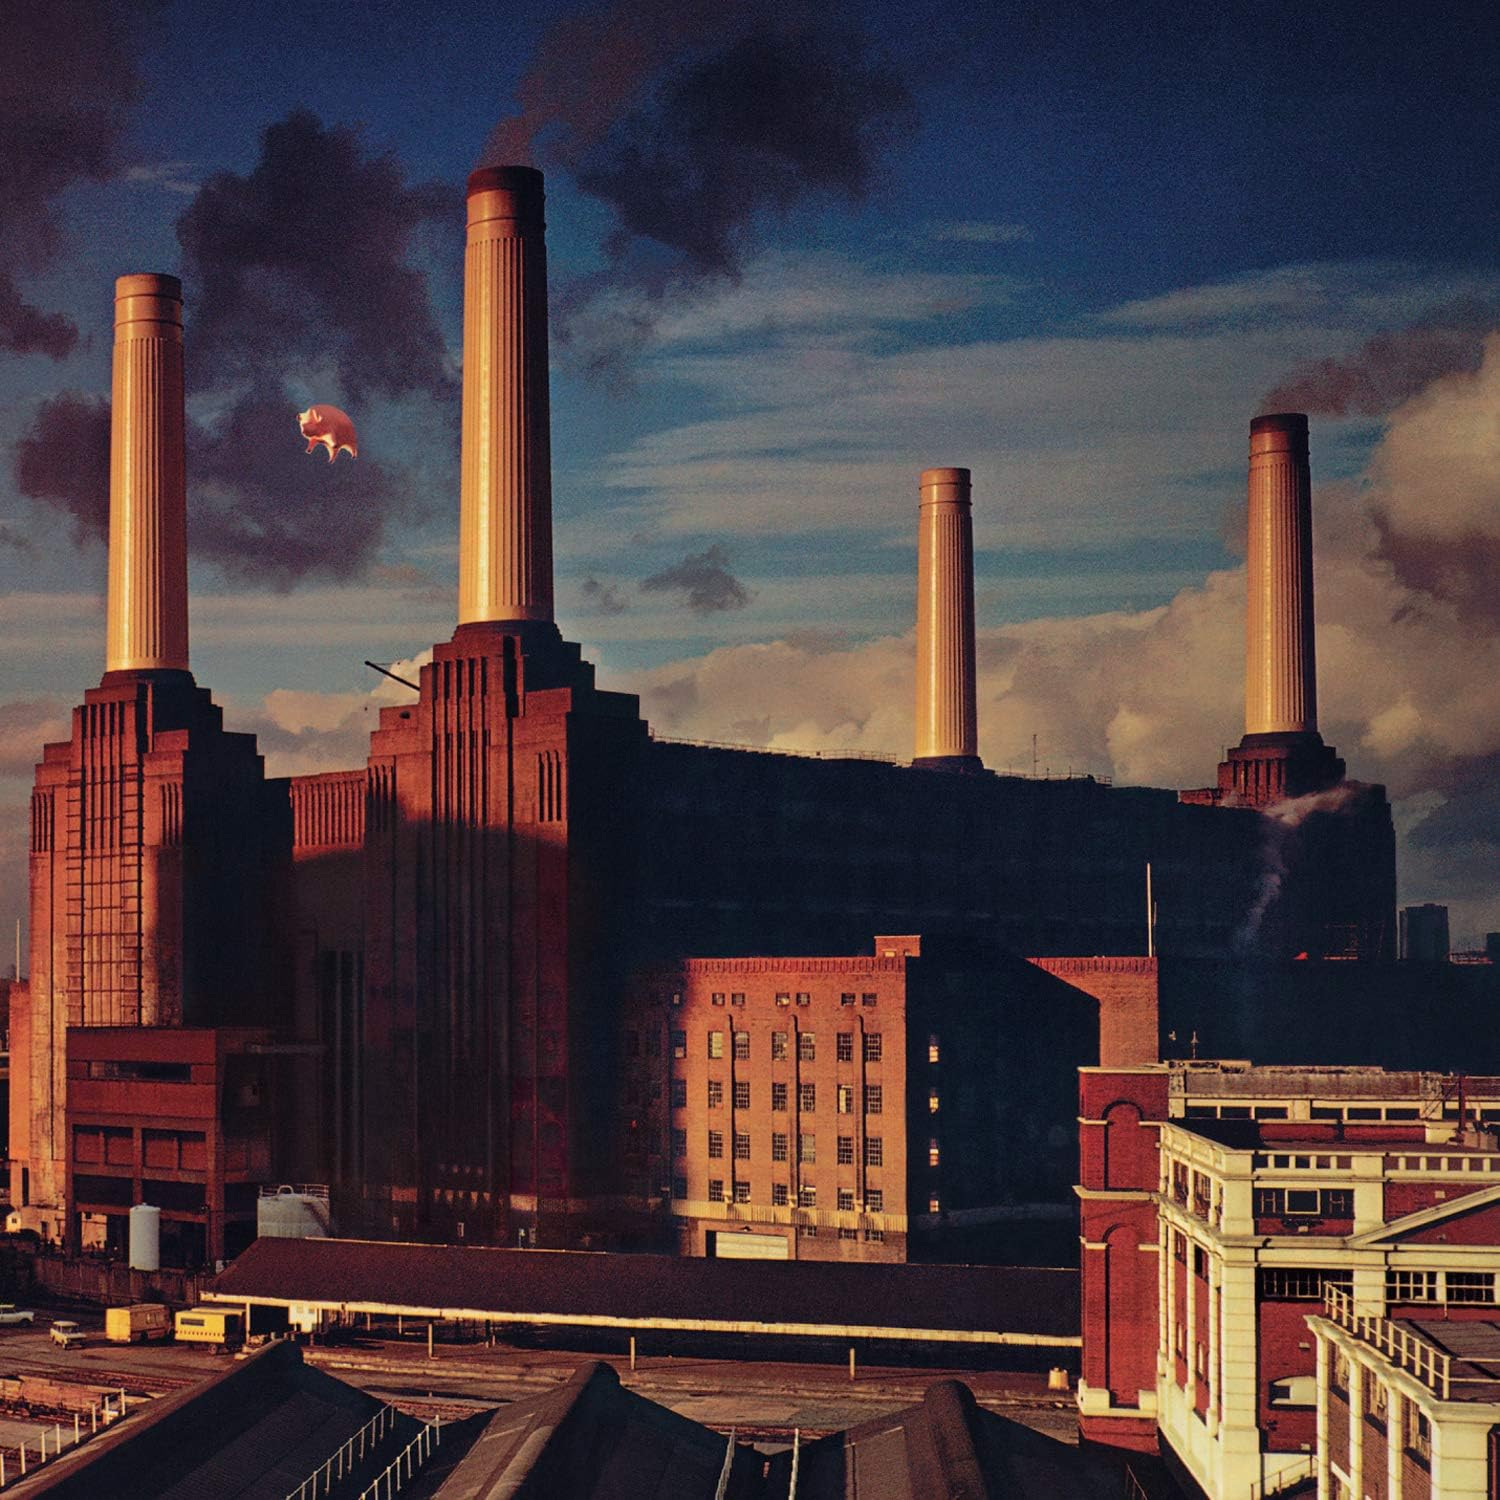
\includegraphics[keepaspectratio,width=.8\textwidth]{cover1977.jpeg}
    %         \label{fig:cover1977}
    %         \subcaption{Release originale.}
    % \end{minipage}
    % \begin{minipage}{.5\textwidth}
    %         \centering
    %         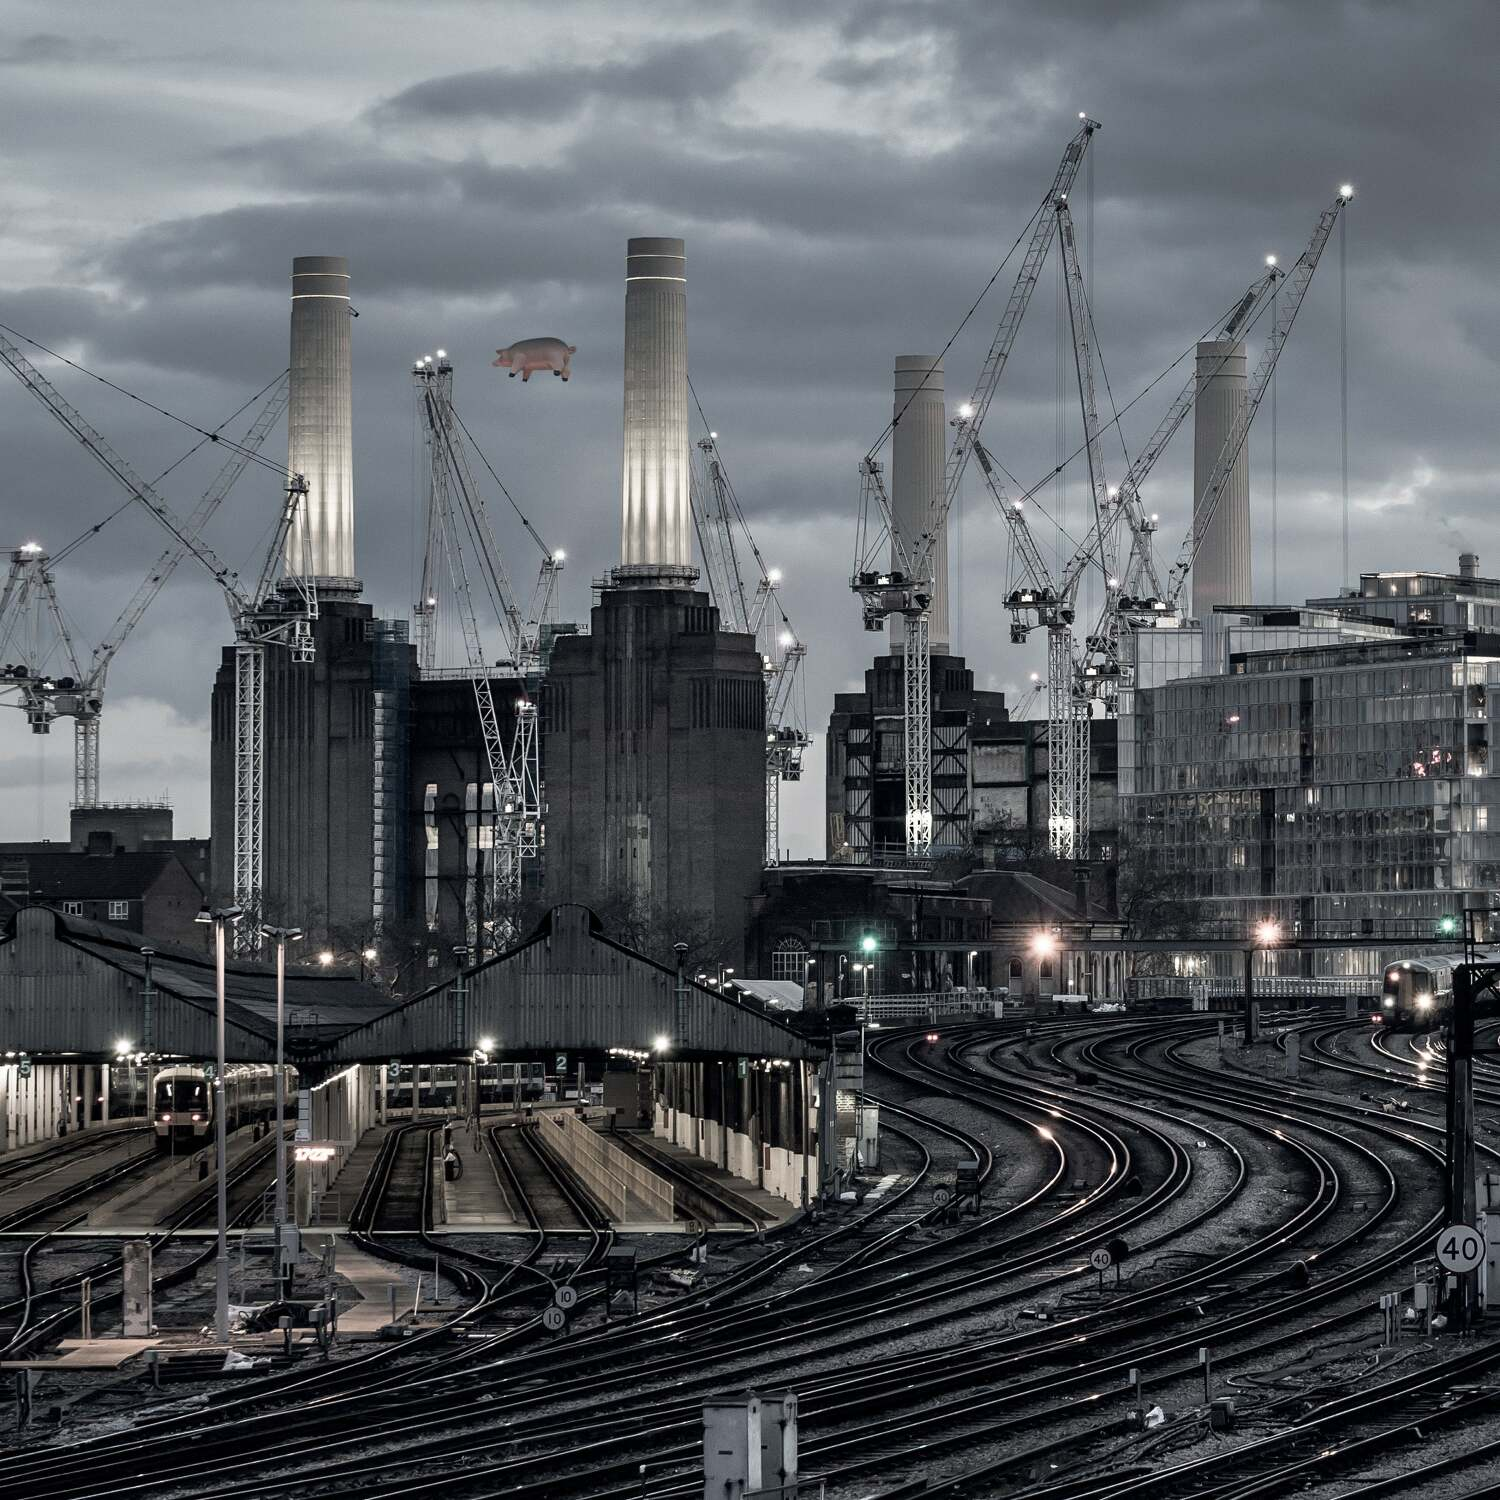
\includegraphics[keepaspectratio,width=.8\textwidth]{cover2018.jpeg}
    %         \label{fig:cover2018}
    %         \subcaption{Remaster 2018.}
    %     \end{minipage}
    %     \caption{Copertina di \acrlong{anm}}
    % \end{figure}
    \begin{figure}[t]
    \centering
        \subfloat[Release originale.]{
                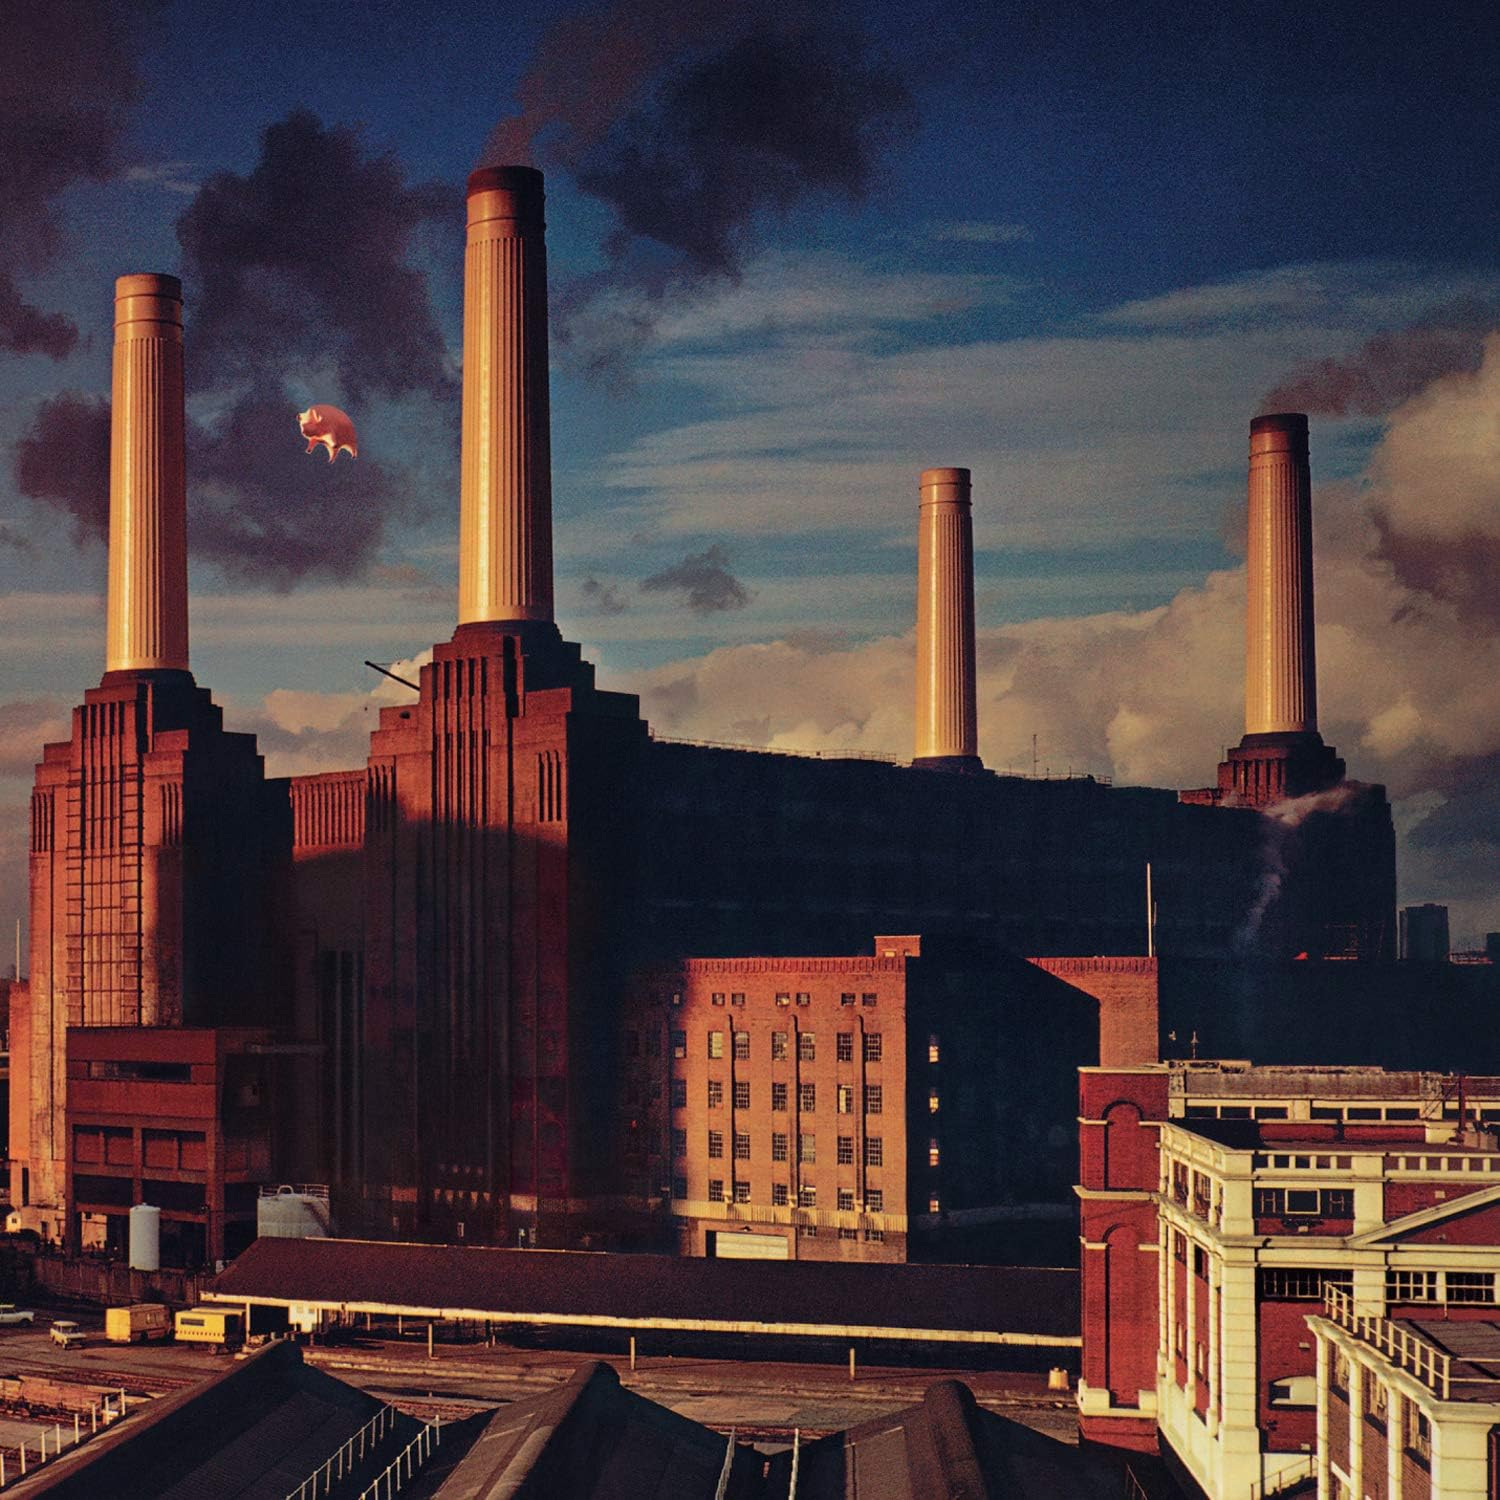
\includegraphics[keepaspectratio,width=.4\textwidth]{cover1977.jpeg}
                \label{fig:cover1977}
                % \subcaption{Release originale.}
            }
        \hspace{.05\textwidth}
        \subfloat[Remaster 2018.]{
                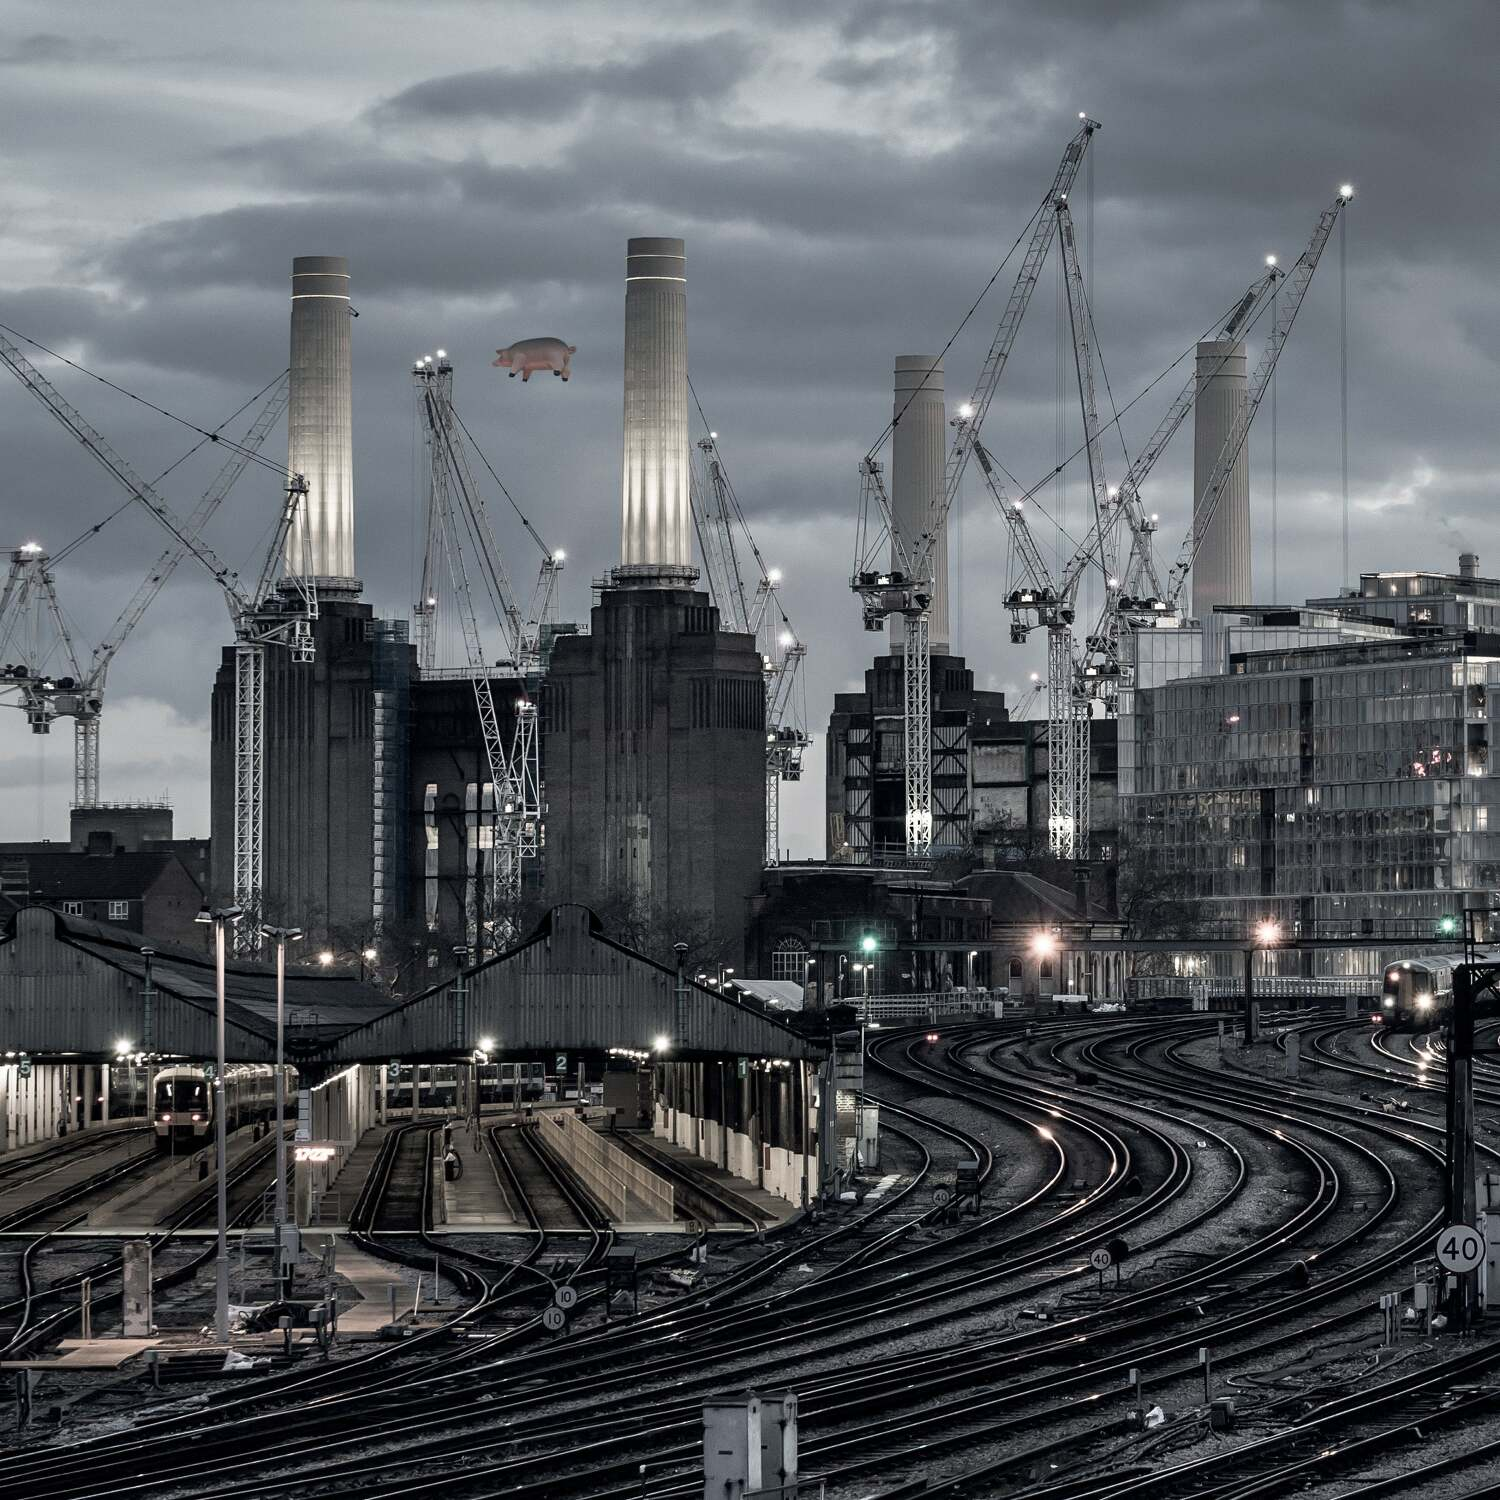
\includegraphics[keepaspectratio,width=.4\textwidth]{cover2018.jpeg}
                \label{fig:cover2018}
                % \subcaption{Remaster 2018.}
            }
        \caption{Copertina di \acrlong{anm}}
    \end{figure}

    \subsection{Tour}
    Il tour promozionale di \acrshort{anm} prese il nome di \emph{In the Flesh tour} e iniziò il giorno stesso del rilascio dell'album. Il tour fu caratterizzato da un'ampia produzione scenica, che includeva un enorme maiale gonfiabile, simile a quello presente in copertina, che volava sopra al pubblico durante i concerti. 

    In supporto del gruppo furono ingaggiati altri musicisti, come il già citato chitarrista Snowy White e il sassofonista Dick Parry, che aveva già ampiamente collaborato con i Floyd durante la produzione e il tour di \acrlong{dsom}, incidendo i soli di \emph{Money} e \emph{Us and Them}.

    Nonostante il grande successo, il tour fu caratterizzato da una crescente tensione all'interno del gruppo, sia a livello individuale, sia a livello relazionale. In particolare, si manifestò in Waters una tendenza all'aggressività nel rapportarsi sia con i colleghi, sia con gli stessi fan durante gli eventi. Questo culminò nella data conclusiva del tour, il 6 luglio presso l'Olympic Stadium di Montreal. Durante l'uscita del gruppo a fine concerto, si creò una piccola calca di fronte al palco  e Waters, in uno scatto d'ira, sputò addosso a uno dei fan. Questo episodio divenne in seguito oggetto di malessere e riflessione profondi per Waters; condividendo questo sentimento con il produttore Bob Ezrin, avrebbe detto di sentire talvolta di aver creato una sorta di barriera tra sé stesso e il pubblico. Questo sentimento di alienazione divenne il nucelo del concept del successivo \acrlong{tw}.
    
    \section{Profilo artistico}\label{sec:02-music}

    \subsection{Concept e tematiche}
    \label{subsec:animals-concept}
    Ispirato al romanzo Animal Farm di George Orwell, l'idea alla base di \acrshort{anm} è la rappresentazione delle classi sociali come  animali: 
    \begin{itemize}
        \item i \emph{cani}, aggressivi, sono i rappresentanti della legge;
        \item i \emph{maiali}, dispotici e spietati, rappresentano i politici;
        \item le \emph{pecore} non sono altro che la mandria insana e cieca che tiene in vita il potere.
    \end{itemize}
    
    L'album, a differenza dell'opera di Orwell, metafora del regime stalinista, è una critica feroce al sistema capitalista nell'Inghilterra degli anni Settanta, e differisce nella rivolta finale delle pecore nei confronti dei cani.

    \subsection{Direzione compositiva}
    \label{subsec:animals-songwriting}
    Sotto il profilo più strettamente musicale, Animals è un album che presenta elementi sia di continuità, sia di rottura con la direzione tracciata dai lavori precedenti. 
    
    Da un lato, infatti, il disco mantiene inalterate la struttura organica e la sinergia tra l'elemento musicale e l'elemento lirico. Delle cinque tracce che costituiscono la tracklist, infatti, la prima e l'ultima fungono  da cornice narrativa, e le tre tracce centrali sono dei brani più lunghi che costituiscono il nucleo centrale dell'album. In questo senso, si può dire che Animals ricalca la stessa struttura adottata dal precedente \acrlong{wywh}; tuttavia, mentre in \acrshort{wywh} il prologo ed epilogo erano costituiti da una lunga \emph{suite} divisa in due parti, in \acrshort{anm} sono due brani molto brevi e semplici in termini di arrangiamento ed esecuzione, e che condividono la medesima struttura armonica e melodica, differendo, di fatto, solo per il testo. 

    \acrshort{anm} mantiene anche molti degli elementi caratteristici del progressive (in salsa) Floyd: i tre brani centrali sono \emph{suite} lunghe e articolate, la ricerca della complessità viene mantenuta tanto nelle scelte armoniche, quanto in quelle melodiche (notevole in questo senso l'uso di una frase armonizzata sulla scala esatonale nel solo di Dogs), gli arrangiamenti sono ricercati e ampio spazio viene riservato alle parti strumentali.

    Dall'altro lato, però, \acrshort{anm} si discosta dai lavori precedenti per alcuni aspetti. In primo luogo, l'album è caratterizzato da un'atmosfera più cupa e tetra rispetto ai precedenti che, in accordo con le tematiche trattate, si riflette nella scelta dei suoni e degli arrangiamenti. In secondo luogo, l'album è caratterizzato da un abbandono delle sonorità affini al \emph{jazz}, molto presenti fino a quel momento e manifestatesi più compiutamente in \acrshort{dsom}, in favore di sonorità \emph{rock} più tradizionali. Questo si declina  in un uso più ampio e marcato della chitarra elettrica e, soprattutto, in una preminenza di tastiere elettromeccaniche (Hammond e Rhodes) a sfavore dei sintetizzatori, che nel precedente \acrshort{wywh} erano protagonisti. Inoltre, i cinque brani che compongono la tracklist possiedono un inizio e una fine ben determinati, in contrasto con la tendenza dei precedenti \acrshort{dsom} e \acrshort{wywh} a presentare brani che si susseguono senza soluzione di continuità. 

    \section{Analisi dei testi}
    \label{sec:02-animals-lyrics}

    \subsection{Pigs on the Wing}
    Il disco si apre con la prima parte di Pigs on the Wing, una breve canzone d'amore che Waters, seppur non dichiaratamente, dedica a sua moglie. La seconda parte di Pigs on the Wing, chiusura dell'album, è strutturalmente e armonicamente  identica alla prima, e differeisce solo per il testo. Mentre la prima parte descrive cosa succederebbe se Waters e la moglie non si curassero l'una dell'altro, la seconda dichiara che ognuno dei due è consapevole dell'amore reciproco. 

    Similmente a quanto avviene in \acrlong{wywh}, il messaggio cupo e disilluso delle altre canzoni viene racchiuso in una cornice in apparenza contrastante per tematica, funzionale a esaltare le crudeltà descritta dal nucleo centrale dell'album e veicolare un messaggio di speranza a cui Waters non riesce a rinunciare. Per affrontare la realtà descritta in quest'album serve amore: prendersi cura del prossimo, interessarsi a cosa gli succede e confidare che anche lui si interessi a te. Il testo parla di unione, estesa a tutti i rapporti umani. Nel legame e nell'aiuto si trova la forza necessaria per trovare riparo dal male, come l'unione di Pigs on the Wing Part 1 e Part 2  è l'unico momento di luce nel buio raccontato in quest'album. Pigs On the Wing ha una domanda sottintesa: cosa succederebbe se non ci importasse l'uno dell'altro? La risposta di Waters è che la vita sarebbe un vagare di sofferenza in sofferenza, chiedendosi inutilmente chi è il colpevole, incapaci di capire che le colpe degli altri iniziano dove finisce la nostra capacità di combatterle. E soprattutto, cosa più importante, vitale per la sopravvivenza, saremmo perennemente in uno stato d'allarme nei confronti di chi ci vuole prevaricare: significherebbe avere paura dei maiali volanti e, visto che i maiali volanti non esistono, angosciarsi per un male illusorio. La parte 2 contiene una netta affermazione, mette in guardia sul possibile rischio di spaventarsi per nemici che non esistono, quando il male è molto più reale.

    Chi è il male, quindi? I cani, tanto per cominciare.

    \subsection{Dogs}
    La prima sezione di Dogs evoca visivamente quelli che sono i meccanismi di un animale randagio: l'allerta costante, il prevaricare i propri simili e il far loro del male senza esitazione se necessario. L'animale in questione non è altro che un imprenditore, che cerca, come un cane per strada, di sopravvivere al mondo capitalista di cui fa parte e che finirà per ridursi a essere soltanto un altro vecchio uomo che si ritrova da solo a morire di "cancro", cioè con il suo senso di colpa che, come un macigno, lo fa sprofondare. In questa parte di testo, l'io narrante si rivolge direttamente al protagonista e la ripetizione delle forme  imperative/esortative \emph{you gotta}, \emph{you have to}, \emph{you can} a inizio del verso (o nella parte iniziale) la rende interpretabile come una serie di istruzioni fornite da un "cane" più esperto a quello più giovane.

    Nella seconda sezione del brano c'è un cambio repentino di punto di vista: la voce narrante esterna viene sostituita dal pronome alla prima persona singolare (\emph{I gotta}), in una narrazione amara e disillusa della propria condizione esistenziale. L'io narrante diventa una figura drammatica, schiacciata come gli altri dal sistema, che cerca di convincersi che anche i rapporti umani siano solo merce sfruttabile e spendibile, che non esista altra logica se non quella del potere.

    Il testo si conclude una stanza di undici versi, ognuno dei quali si apre con la formula who was, che non fa altro che inglobare quella che è la vita del protagonista, che sembra, attraverso la formulazione impersonale, la descrizione di una tragedia condivisa destinata a ripetersi all'infinito. Sono interessanti, dal punto di vista lirico, le assonanze e le rime che si vanno a creare "in mezzo al verso" (per esempio born-told; ground-found). È da rimarcare l'importanza delle ripetizioni a inizio verso che caratterizzano tutta la canzone, quasi a voler riprodurre il senso di affanno di questa lotta inutile

    \subsection{Pigs (Three Different Ones)}pigs
    In posizione centrale all'album troviamo \acrfull{p}, che non a caso tratta di quello che è il centro del potere nella narrativa di Animals: i maiali, che controllano le pecore, ma anche i cani. Questi ultimi, in particolare, li favoriscono con le proprie azioni ma al tempo stesso li devono temere, perché i maiali all'apparenza possono vedere tutto e fare tutto, anche volare (questo concetto viene esplicitato negli ultimi versi di \acrshort{pw2}). I maiali sono metafora della corruzione, dello sfruttamento, del potere apparentemente illimitato di chi sta ai vertici, ma che non è altro che una farsa ridicola di figure ridicole, portata alla luce già nei primi versi della canzone (\emph{Ha ha, charade you are}). A differenza del tono claustrofobico e cupo di \acrshort{d}, \acrshort{p} è una canzone più spigliata e che usa il sarcasmo come propria arma di difesa: ogni strofa si conclude con "You're nearly a laugh/a treat but you're really a cry" a sottolineare come la grettezza di questi individui sia così triste da suscitare ilarità, una risata, esorcizzando il tutto mediante l'ironia. 
    
    Il brano è diviso in tre strofe, in ognuna delle quali viene presentato un tipo differente di maiale:

    \paragraph{Prima strofa} Qui Waters si rivolge in generale agli uomini di potere e alle grandi lobby (well heeled big wheel). L'idea del personaggio è resa dall'immagine del maiale che mangia dal bidone mentre ordina agli altri di continuare a scavare, in modo da procurargli più cibo. Gli appellativi e le immagini selezionate per descrivere il maiale (\emph{Big man, pig man; joker; pig stain on your fat chin} etc.) enfatizzano la natura grottesca del personaggio, altrettanto moralmente ripugnante.

    \paragraph{Seconda strofa} Il secondo maiale è la figura del politico. Anche se non confermato, l'appellativo \emph{"old hag"} e i versi \emph{"you like the feel of steel"} e "and good fun with a hand gun" sembrano riferirsi a Margareth Thatcher. Anche in questo caso l'io narrante si rivolge al personaggio con termini ridicolizzanti (\emph{bus stop rat bag, fucked up old hag, hot stuff with a hatpin}) e attaccando la sua presunta integrità istituzionale (\emph{you radiate shafts of broken glass}). L'utilizzo di termini più gergali sembra inasprire la critica e marcare la distanza che si percepisce tra la classe dirigente, in questo caso conservatrice e di stampo borghese, e la gente comune.

    \paragraph{Terza strofa} L'ultimo strofa, invece, è un attacco diretto e inequivocabile all'attivista moralizzatrice \emph{Mary Whitehouse}. Si tratta di gran lunga della critica più dura del brano, essendo il terzo maiale la rappresentazione di quel potere latente e strisciante più difficile da arginare: l'influenza dei media e dell'attivismo nocivo. In particolare, nei versi "You're trying to keep our feelings off the street" e"Gotta stem the evil tide and keep it all inside"(dove cita la stessa attivista), Waters sembra riferirsi all'episodio del bando per "oscenità" del Little Red Schoolbook\footnote{rivista/guida per giovani sul sesso, sugli stupefacenti e sugli atteggiamenti degli adulti}, avvenuto a seguito della forte polemica mediatica della Whitehouse. Per la sua continua lotta contro le "oscenità", che lei vedeva come un'ossessione, Waters la definisce incapace di provare piacere sessuale (tight lips) e terribilmente sola (cold feet). L'affondo di Waters continua chiedendole se per caso è stata oggetto di abusi quando era bambina: "And do you feel abused?, seguito da ansimi inequivocabili. A differenza delle altre due strofe, nei versi conclusivi le si rivolge appellandola col nome proprio, come a voler demolire il potere datole dalla sua influenza mediatica, e ridurla a una semplice "Mary".

    \subsection{Sheep}
    A seguire Pigs è un'atmosfera agreste in cui si sentono pecore che belano e uccelli che cinguettano. Si tratta dell'inizio della canzone Sheep, che completa il nucleo centrale dell'album e introduce al terzo protagonista del concept: le pecore.

    Le pecore rappresentano le masse, mancanti di pensiero critico e per questo incapaci di uscire dal recinto costruito dai maiali e dai cani per confinarle e renderle innocue. Queste trascorrono la vita pascolando per mangiare, dormire e riprodursi, con la vaga sensazione che c'è qualcosa di sbagliato nella società in cui vivono, ma senza la forza né il coraggio di capire che cosa sia. Al di là dei loro bisogni primari vedono poco e pensano ancora meno, e sarà sui bisogni primari che il potere batterà il chiodo per garantire che queste persone stiano dalla loro parte (what do you get pretending \([\ldots]\)?). La pecora è, nell'immaginario religioso, simbolo di candida innocenza; la frase "I've looked over Jordan and I have seen things are not what they seem" può significare che la realtà può essere terribilmente diversa da come appare a chi la vede con gli occhi di una fede, sia questa religiosa o di altra natura, come nelle istituzioni o in una persona vista come "guida". Le pecore fingono di non essere in pericolo e seguono fedelmente il leader. Quando la realtà, inevitabilmente, si mostrerà per com'è veramente ("Now things are really what they seem"), si sorprenderanno di non essere in un incubo.

    Dopo un riecheggiare della grido "stone" da Dogs, Waters recita una sorta di preghiera con voce distorta, incomprensibile. L'idea è sempre proporre il linguaggio alieno delle "pecore" della società

    \begin{itemize}
        \item Dal punto di vista musicale, la strofa è una cieca litania, inquietante e priva di colore, dove la voce è accompagnata da una lunga serie di suoni metallici che si mescolano con gli effetti del sintetizzatore e del basso. Il sermone inizia blando ma viene contagiato dal ritmo incalzante della canzone, ben presto il belare ossessivo delle pecore diventa assordante, si sormonta alla voce che continua a pronunciare suoni senza senso finché tutto finisce com'era iniziata, improvvisamente, con la terza strofa cantata
        \item Liricamente parlando, il delirio sonoro viene tradotto testo che comunica perfettamente la condizione di folle schiavitù in cui vivono le pecore. Il finto sermone di Waters ricalca il Salmo 23 dell' Antico Testamento, il che consente di rendere anche nel testo la sensazione di ridondanza che facilita la memorizzazione durante la recitazione. Il contenuto è stravolto e adattato narrativamente alla voce dei  "fedeli", una massa che è disposta ad accettare qualsiasi forma di limitazione della libertà (I shall not want) e crudeltà (/he maketh me to hang on hooks in high places/) in cambio dei piaceri effimeri a lei concessi, anche i più ridicoli.
    \end{itemize}

    Il potere usa la religione e la politica per controllare le masse che potrebbero ribellarsi, come succede nel finale del brano, dove le pecore si rivoltano contro i padroni (i cani), con un grido. Questo verso può avere una seconda interpretazione, cioè il gettarsi al collo di qualcuno in un cieco atto di devozione. Le pecore sono tante da sembrare un esercito, vanno tutte nella stessa direzione come ogni gregge, ammasso mobile e folle (demented avengers) che crede di essere uscito finalmente dalle tenebre e avviato all'interno del sogno (la loro presunta libertà).

    Nell'ultima strofa, i cani sono morti sotto la rivolta delle pecore. Ma non è che un mero ribaltamento di potere: alcune pecore esultanti intimano ad altre pecore di "restare nelle loro case e fare ciò che viene detto loro" rimarcando come la loro natura di sottomissione non possa mai cambiare.

\end{document}